\documentclass{standalone}
%
\usepackage{tikz}
%
\usepackage{fontspec}
\setmainfont{Montserrat}
%
\title{Squares}
\begin{document}
	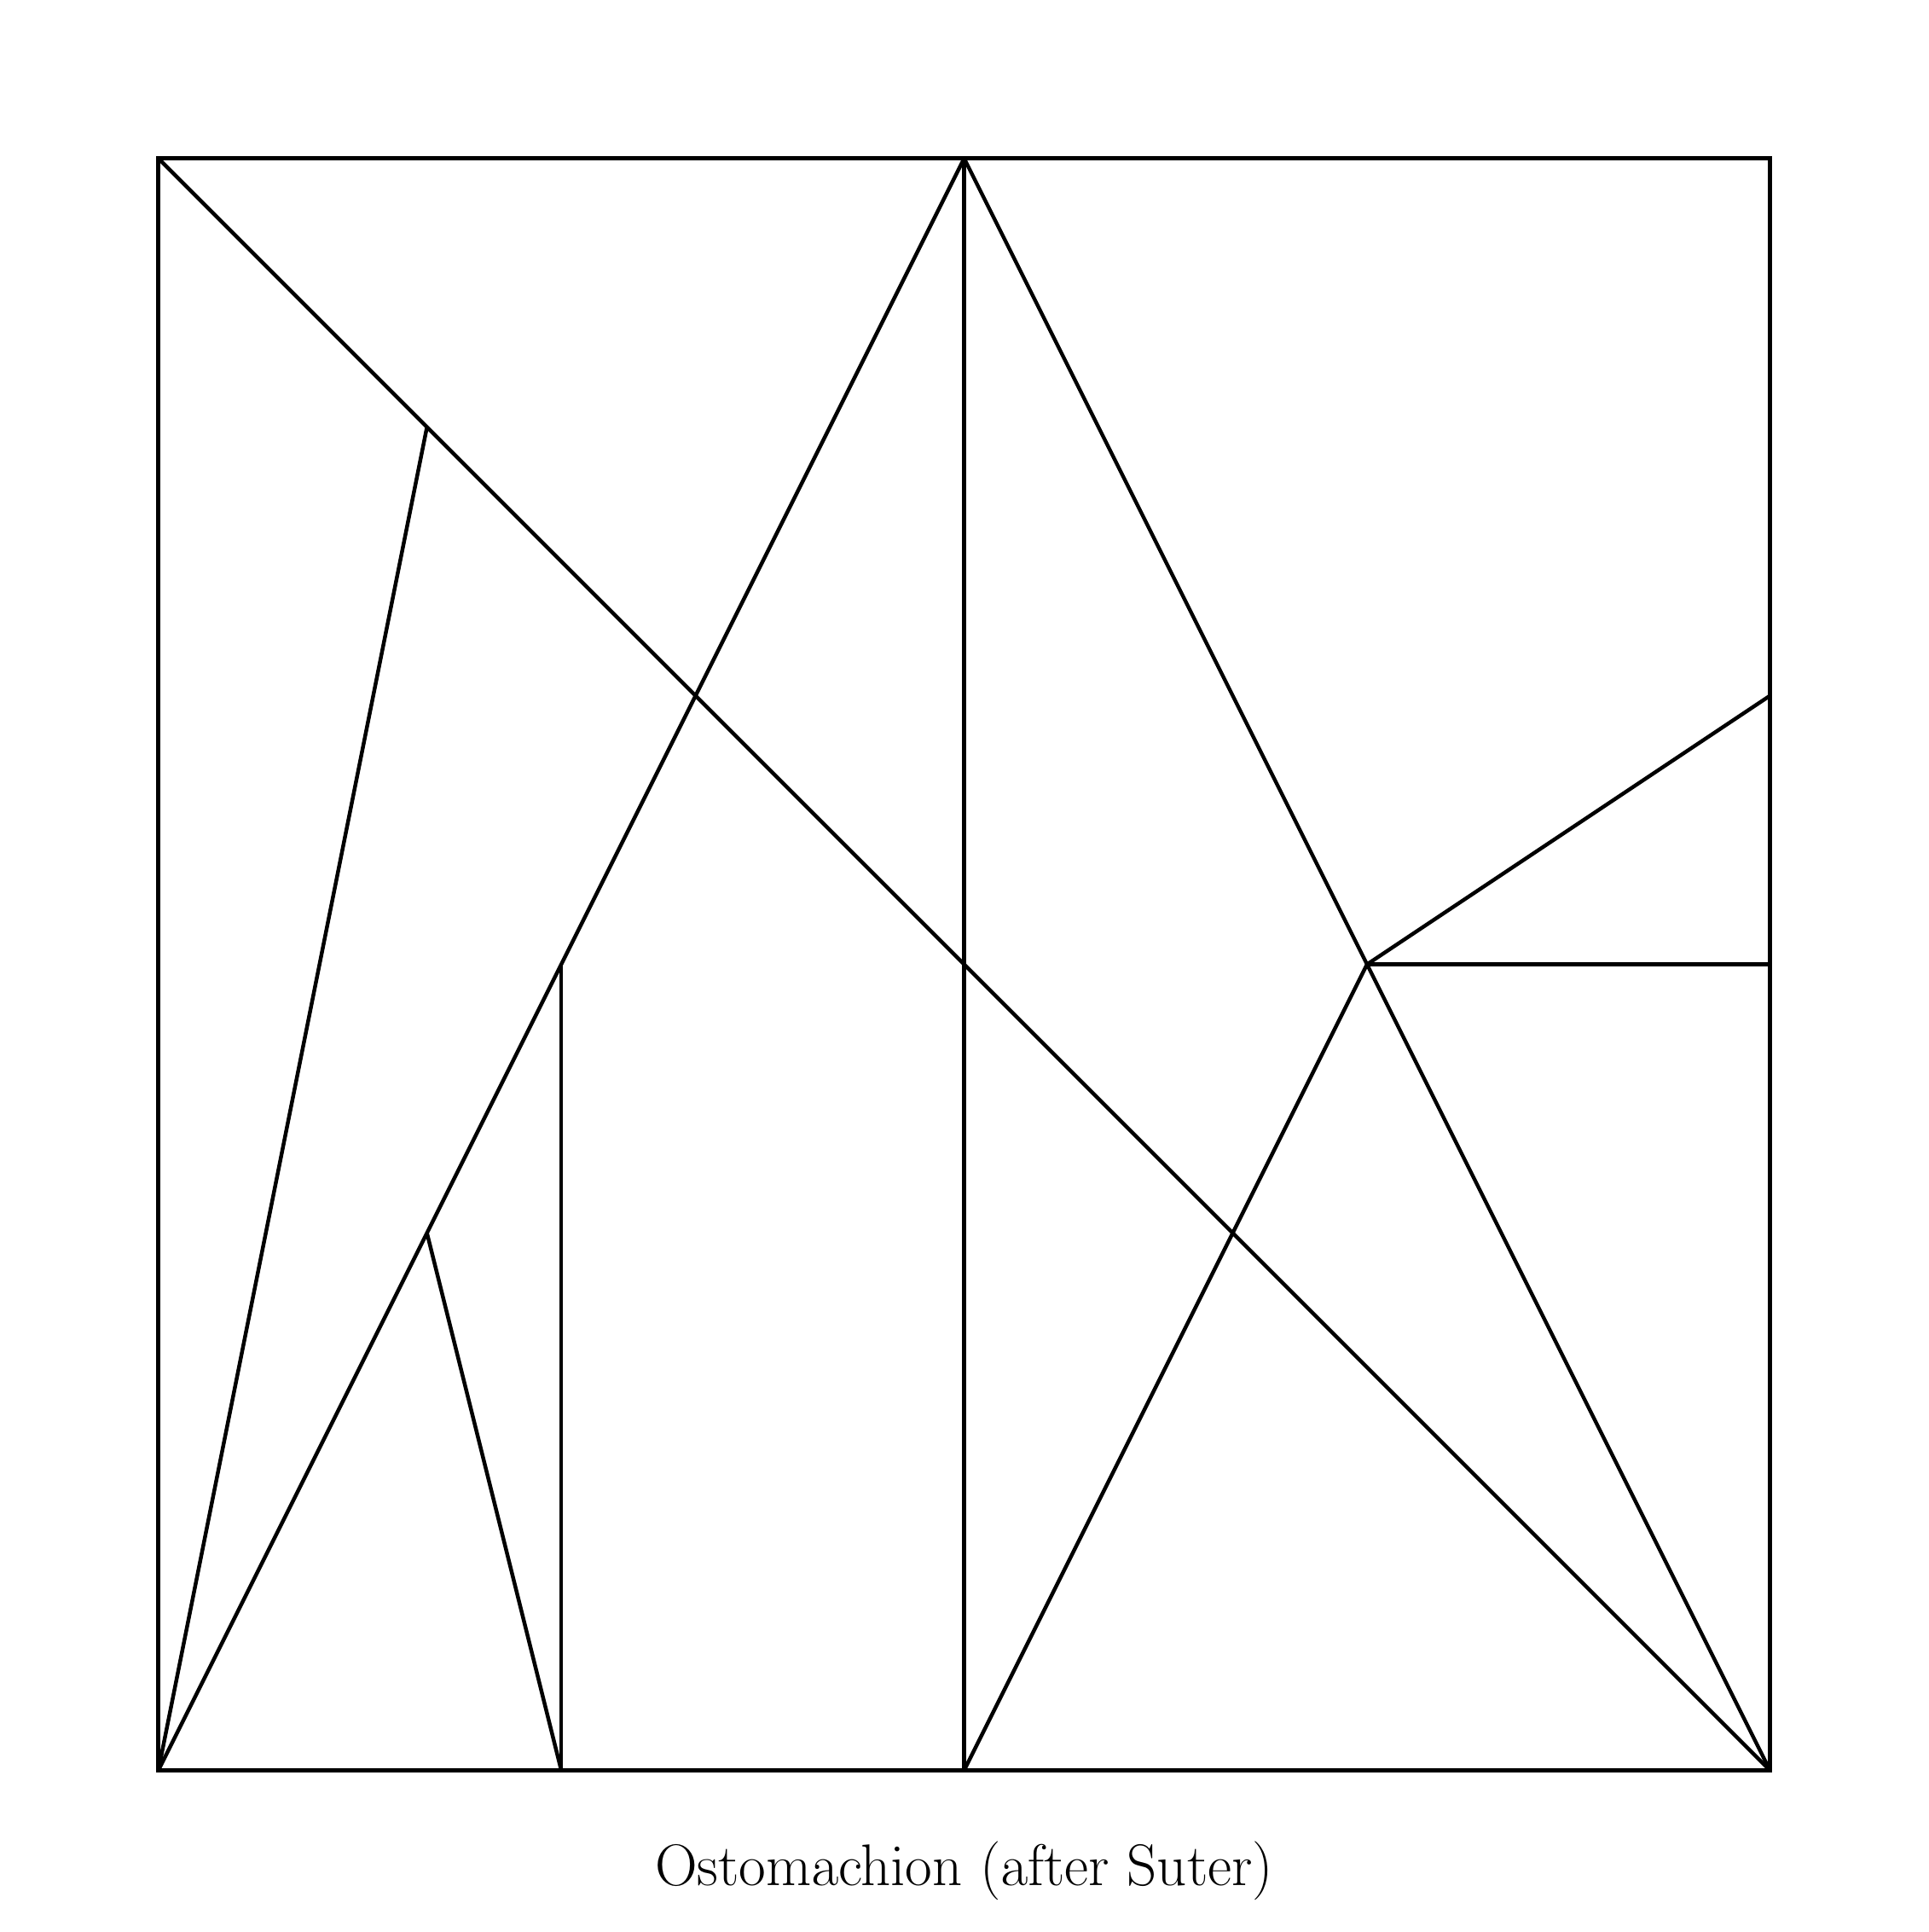
\begin{tikzpicture}
		\begin{scope}[scale=2]
			\draw [color=white,fill=white] (-1,1) rectangle (13,-13);
			\draw [ultra thick] (0,0) rectangle (12,-12);
			\draw [ultra thick] (0,0) -- (12,-12);
			\draw [ultra thick] (0,-12) -- (2,-2);
			\draw [ultra thick] (6,0) -- (6,-12);
			\draw [ultra thick] (6,0) -- (12,-12);
			\draw [ultra thick] (6,-12) -- (9,-6);
			\draw [ultra thick] (9,-6) -- (12,-6);
			\draw [ultra thick] (9,-6) -- (12,-4);
			\draw [ultra thick] (0,-12) -- (6,0);
			\draw [ultra thick] (3,-6) -- (3,-12);
			\draw [ultra thick] (2,-8) -- (3,-12);
		\end{scope}
		%
		\begin{scope}[shift={(0,-25.5)}]
			\node at (12,0) {\textcolor{black}{\fontsize{27}{28}\selectfont Ostomachion (after Suter)}};
		\end{scope}
	\end{tikzpicture}
\end{document}